\documentclass[12pt]{report}
\usepackage[utf8]{inputenc}
\usepackage[russian]{babel}
%\usepackage[14pt]{extsizes}
\usepackage{listings}
\usepackage{xcolor}

% Для листинга кода:
\lstset{ %
	language= C,                 % выбор языка для подсветки 
	basicstyle=\small\sffamily, % размер и начертание шрифта для подсветки кода
	numbers=left,               % где поставить нумерацию строк (слева\справа)
	numberstyle=\tiny,           % размер шрифта для номеров строк
	stepnumber=1,                   % размер шага между двумя номерами строк
	numbersep=5pt,                % как далеко отстоят номера строк от подсвечиваемого кода
	showspaces=false,            % показывать или нет пробелы специальными отступами
	showstringspaces=false,      % показывать или нет пробелы в строках
	showtabs=false,             % показывать или нет табуляцию в строках            
	tabsize=2,                 % размер табуляции по умолчанию равен 2 пробелам
	captionpos=t,              % позиция заголовка вверху [t] или внизу [b] 
	breaklines=true,           % автоматически переносить строки (да\нет)
	breakatwhitespace=false, % переносить строки только если есть пробел
	escapeinside={\#*}{*)}   % если нужно добавить комментарии в коде
}

\definecolor{comment}{RGB}{0,128,0} % dark green
\definecolor{string}{RGB}{255,0,0}  % red
\definecolor{keyword}{RGB}{0,0,255} % blue

\lstdefinestyle{CStyle}{
	commentstyle=\color{comment},
	stringstyle=\color{string},
	keywordstyle=\color{keyword},
	basicstyle=\footnotesize\ttfamily,
	numbers=left,
	numberstyle=\tiny,
	numbersep=5pt,
	frame=lines,
	breaklines=true,
	prebreak=\raisebox{0ex}[0ex][0ex]{\ensuremath{\hookleftarrow}},
	showstringspaces=false,
	upquote=true,
	tabsize=2,
}

% Для измененных титулов глав:
\usepackage{titlesec, blindtext, color} % подключаем нужные пакеты
\definecolor{gray75}{gray}{0.75} % определяем цвет
\newcommand{\hsp}{\hspace{20pt}} % длина линии в 20pt
% titleformat определяет стиль
\titleformat{\chapter}[hang]{\Huge\bfseries}{\thechapter\hsp\textcolor{gray75}{|}\hsp}{0pt}{\Huge\bfseries}

%отступы по краям
\usepackage{geometry}
\geometry{verbose, a4paper,tmargin=2cm, bmargin=2cm, rmargin=1.5cm, lmargin = 3cm}
% межстрочный интервал
\usepackage{setspace}
\onehalfspacing
\usepackage{float}
% plot
\usepackage{pgfplots}
\usepackage{filecontents}
\usepackage{amsmath}
\usepackage{tikz,pgfplots}
\usetikzlibrary{datavisualization}
\usetikzlibrary{datavisualization.formats.functions}

\usepackage{graphicx}
\graphicspath{{src/}}
\DeclareGraphicsExtensions{.pdf,.png,.jpg}

\usepackage{geometry}
\geometry{verbose, a4paper,tmargin=2cm, bmargin=2cm, rmargin=1.5cm, lmargin = 3cm}
\usepackage{indentfirst}
\setlength{\parindent}{1.4cm}

\usepackage{titlesec}
\titlespacing{\chapter}{0pt}{12pt plus 4pt minus 2pt}{0pt}


\begin{document}
%\def\chaptername{} % убирает "Глава"
\begin{titlepage}
	\centering
	{\scshape\LARGE МГТУ им. Баумана \par}
	\vspace{3cm}
	{\scshape\Large Лабораторная работа №5\par}
	\vspace{0.5cm}	
	{\scshape\Large По курсу: "Операционные системы"\par}
	\vspace{1.5cm}
	\centering
	 {\huge\bfseries Взаимодействие параллельных процессов.\par}
	\vspace{2cm}
	\Large Работу выполнил: Мокеев Даниил, ИУ7-56\par
	\vspace{0.5cm}
	\Large Преподаватель:  Рязанова Н.Ю.\par

	\vfill
	\large \textit {Москва, 2020} \par
\end{titlepage}


\newpage

\section{Листинг кода алгоритмов}
В данном разделе будут приведены листинги кода реализованных программ. 

\begin{lstlisting}[label=one,caption = Задача производства-потребления, style = CStyle]
#include <signal.h>
#include <stdio.h>
#include <stdlib.h>
#include <sys/stat.h>
#include <sys/sem.h>
#include <sys/shm.h>
#include <time.h>
#include <unistd.h>
#include <sys/wait.h>

#define SEM_BIN   0
#define SEM_EMPTY 1
#define SEM_FULL  2

#define P -1
#define V 1

#define PRODUCERS_COUNT 3
#define CONSUMERS_COUNT 3

#define BUFFER_SIZE 3

#define PERMS S_IRWXU | S_IRWXG | S_IRWXO //permition to read, write & execute by user, group & others

#define COMSUMER_BORDER "\t\t\t\t\t\t"

int sem_id = -1;
int shm_id = -1;

int *shm = NULL;
int *shm_pos = NULL;
int *produced_value = NULL;
int *last_consumed = NULL;

struct sembuf producer_start[2] = {
	{SEM_EMPTY, P, SEM_UNDO},
	{SEM_BIN,   P, SEM_UNDO}
};
struct sembuf producer_stop[2] = {
	{SEM_BIN,   V, SEM_UNDO},
	{SEM_FULL,  V, SEM_UNDO}
};

struct sembuf consumer_start[2] = {
	{SEM_FULL,  P, SEM_UNDO},
	{SEM_BIN,   P, SEM_UNDO}
};
struct sembuf consumer_stop[2] = {
	{SEM_BIN,   V, SEM_UNDO},
	{SEM_EMPTY, V, SEM_UNDO}
};

void fork_children(const int n, void (*func)(const int)) {
	for (int i = 0; i < n; ++i) {
		const pid_t pid = fork();
		
		if (pid == -1) {
			perror("fork");
			exit(1);
		} else if (pid == 0) {
			if (func) {
				func(i);
			}
			exit(1);
		}
	}
}

void wait_children(const int n) {
	for (int i = 0; i < n; ++i) {
		int status;
		const pid_t child_pid = wait(&status);
		if (child_pid == -1) {
			perror("wait error");
			exit(1);
		}
		
		if (WIFEXITED(status)) {
			printf("Process %d returns %d\n", child_pid, WEXITSTATUS(status));
		} else if (WIFSIGNALED(status)) {
			printf("Process %d terminated with signal %d\n", child_pid, WTERMSIG(status));
		} else if (WIFSTOPPED(status)) {
			printf("Process %d stopped due signal %d\n", child_pid, WSTOPSIG(status));
		}
	}
}

void producer(const int id) {
	while(1) {
		sleep(rand() % 3);
		
		if(*produced_value > 122)
		exit(0);
		
		if (semop(sem_id, producer_start, 2) == -1) {
			perror("semop");
			exit(1);
		}
		
		// write next value in shared memory
		*(shm + *shm_pos) = *produced_value;
		printf("Producer %d (pid %d) produces %c\n", id, getpid(), *produced_value);
		(*shm_pos)++;
		(*produced_value)++;
		
		if (semop(sem_id, producer_stop, 2) == -1) {
			perror("semop");
			exit(1);
		}
		
	}
}

void consumer(const int id) {
	while(1) {
		sleep(rand() % 2);
		
		if (*last_consumed >= 122)
		exit(0);
		
		if (semop(sem_id, consumer_start, 2) == -1) {
			perror("semop");
			exit(1);
		}
		
		printf(COMSUMER_BORDER"Consumer %d (pid %d) consumes %c\n", id, getpid(), *(shm +(*shm_pos)-1));
		*(last_consumed) = *(shm +(*shm_pos)-1);
		(*shm_pos)--;
		
		if (semop(sem_id, consumer_stop, 2) == -1) {
			perror("semop");
			exit(1);
		}
	}
}


void init_semaphores() {
	sem_id = semget(IPC_PRIVATE, 3, IPC_CREAT | PERMS);
	if (sem_id == -1) {
		perror("semget");
		exit(1);
	}
	if (semctl(sem_id, SEM_BIN,   SETVAL, 1) == -1 ||
	semctl(sem_id, SEM_EMPTY, SETVAL, BUFFER_SIZE) == -1 ||
	semctl(sem_id, SEM_FULL,  SETVAL, 0) == -1) {
		perror("semctl");
		exit(1);
	}
}

void init_shared_memory() {
	shm_id = shmget(IPC_PRIVATE, (BUFFER_SIZE+3) * sizeof(int), IPC_CREAT | PERMS);
	
	if (shm_id == -1) {
		perror("shmget");
		exit(1);
	}
	shm = shmat(shm_id, 0, 0);
	if (shm == (void *) -1) {
		perror("shmat");
		exit(1);
	}
	
	shm_pos = shm;
	*shm_pos = 0;
	produced_value = shm+2;
	last_consumed = shm+1;
	
	*produced_value = 97;
	*last_consumed = 97;
	shm = shm + 3;
	
}

int main() {
	int children = 0;
	srand((unsigned int) time(NULL));
	
	init_semaphores();
	init_shared_memory();
	
	fork_children(PRODUCERS_COUNT, producer);
	fork_children(CONSUMERS_COUNT, consumer);
	
	wait_children(PRODUCERS_COUNT + CONSUMERS_COUNT);
	
	shmctl(shm_id, IPC_RMID, NULL);
	semctl(sem_id, SEM_BIN, IPC_RMID, 0);
}

\end{lstlisting}
\begin{figure}[H]
	\centering{\includegraphics[scale=0.6]{image/task1-start.png}} 
	\caption{Пример работы программы. BUFFER\textunderscore SIZE = 3 (начало вывода)}
	\label{ris:1}
\end{figure}

\begin{figure}[H]
	\centering{\includegraphics[scale=0.6]{image/task1-finish.png}} 
	\caption{Пример работы программы. BUFFER\textunderscore SIZE = 3 (конец вывода)}
	\label{ris:2}
\end{figure}

\newpage
\begin{lstlisting}[label=two,caption = Задача читатели-писатели, style = CStyle]
#include <sys/shm.h>
#include <sys/sem.h>
#include <fcntl.h>
#include <unistd.h>
#include <sys/wait.h>
#include <stdio.h>
#include <stdlib.h>
#include <signal.h>
#include <time.h>

#define READER_BORDER "\t\t\t\t\t\t"

#define PERMS S_IRWXU | S_IRWXG | S_IRWXO

#define MAX_VALUE 10
#define WRITERS 3
#define READERS 5

#define ACTIVE_WR 0
#define ACTIVE_RR 1
#define WAITING_W 2
#define WAITING_R 3

#define V 1
#define P -1
#define Z 0

#define SEM_ACTIVE_WR 0
#define SEM_ACTIVE_RR 1
#define SEM_WAITING_W 2
#define SEM_WAITING_R 3

struct sembuf start_reading[] = {
	{SEM_WAITING_R, V, SEM_UNDO},
	{SEM_ACTIVE_WR, Z, SEM_UNDO},
	{SEM_WAITING_W, Z, SEM_UNDO},
	{SEM_ACTIVE_RR, V, SEM_UNDO},
	{SEM_WAITING_R, P, SEM_UNDO}
};
struct sembuf stop_read[] = {
	{SEM_ACTIVE_RR, P, SEM_UNDO}
};

struct sembuf start_writing[] = {
	{SEM_WAITING_W, V, SEM_UNDO},
	{SEM_ACTIVE_RR, Z, SEM_UNDO},
	{SEM_ACTIVE_WR, Z, SEM_UNDO},
	{SEM_ACTIVE_WR, V, SEM_UNDO},
	{SEM_WAITING_W, P, SEM_UNDO}
};
struct sembuf stop_write[] = {
	{SEM_ACTIVE_WR, P, SEM_UNDO}
};

int *shared_value;

pid_t *child_pids;


void kill_writers() {
	for (int i = 0; i < WRITERS; i++) {
		if (child_pids[i] == getpid()) {
			continue;
		}
		kill(child_pids[i], SIGTERM);
	}
}

int init_sh_mem() {
	int fd = shmget(IPC_PRIVATE, sizeof(int), IPC_CREAT | PERMS);
	if (fd == -1) {
		perror("shmget");
		exit(1);
	}
	return fd;
}

int *get_sh_mem_addr(const int fd) {
	int *addr = (int *) shmat(fd, NULL, 0);
	if (addr == (int *) -1) {
		perror("shmat error");
		exit(1);
	}
	return addr;
}

int init_semaphores() {
	int semid = semget(IPC_PRIVATE, 4, IPC_CREAT | PERMS);
	if (semid == -1) {
		perror("semget error");
		exit(1);
	}
	
	int mem_ctrl    = semctl(semid, WAITING_R, SETVAL, 0);
	int writer_ctrl = semctl(semid, ACTIVE_WR, SETVAL, 0);
	int reader_ctrl = semctl(semid, ACTIVE_RR, SETVAL, 0);
	int wait_ctrl   = semctl(semid, WAITING_W, SETVAL, 0);
	
	if (mem_ctrl == -1 || writer_ctrl == -1 || reader_ctrl == -1 || wait_ctrl == -1) {
		perror("semctl");
		exit(1);
	}
	
	return semid;
}

void writer(int semid, int number) {
	int can = semop(semid, start_writing, 5);
	if (can == -1) {
		perror("semop start writing error");
		exit(1);
	}
	// Z condition for stopping all writers
	if (*shared_value >= MAX_VALUE) {
		kill_writers();
		int sem_op_stop = semop(semid, stop_write, 1);
		if (sem_op_stop == -1) {
			perror("semop stor write error");
			exit(1);
		}
		exit(0);
	}
	// write
	(*shared_value)++;
	printf("Writer #%d, pid=%d wrote value %d\n", number, getpid(), *shared_value);
	
	int sem_op_stop = semop(semid, stop_write, 1);
	if (sem_op_stop == -1) {
		perror("semop stop_write");
		exit(1);
	}
	
	sleep(rand() % 10);
}

void reader(int semid, int number) {
	int can = semop(semid, start_reading, 5);
	if (can == -1) {
		perror("semop start_reading");
		exit(1);
	}
	// read
	int val = *shared_value;
	printf(READER_BORDER"Reader #%d, pid=%d read value: %d\n", number, getpid(), val);
	
	int sem_op_stop = semop(semid, stop_read, 1);
	if (sem_op_stop == -1) {
		perror("semop stop_read");
		exit(1);
	}
	// Z condition for stopping all readers
	if (val >= MAX_VALUE) {
		exit(0);
	}
	
	sleep(rand() % 10);
}

void init_writer(int number, int sem_id) {
	pid_t pid;
	
	if ((pid = fork()) == -1) {
		printf("Can't fork");
		exit(1);
	}
	
	if (pid == 0) {
		printf("Writer #%d created, pid: %d\n", number, getpid());
		while (1) {
			writer(sem_id, number);
		}
	}
	else {
		child_pids[number] = pid;
	}
}

void init_reader(int number, const int sem_id) {
	pid_t pid;
	
	if ((pid = fork()) == -1) {
		printf("Can't fork");
		exit(1);
	}
	
	if (pid == 0) {
		printf(READER_BORDER"Reader #%d created, pid: %d\n", number, getpid());
		while (1) {
			reader(sem_id, number);
		}
	}
	else {
		child_pids[WRITERS + number] = pid;
	}
}

int main() {
	int sh_mem_fd = init_sh_mem();
	int *sh_mem = get_sh_mem_addr(sh_mem_fd);
	
	shared_value = sh_mem;
	*shared_value = 0;
	child_pids = shared_value + 1;
	
	int semid = init_semaphores();
	
	for (int i = 0; i < WRITERS; i++) {
		init_writer(i, semid);
	}
	
	for (int i = 0; i < READERS; i++) {
		init_reader(i, semid);
	}
	
	for (int i = 0; i < WRITERS + READERS; i++) {
		int *status;
		wait(status);
	}
}
\end{lstlisting}

\begin{figure}[H]
	\centering{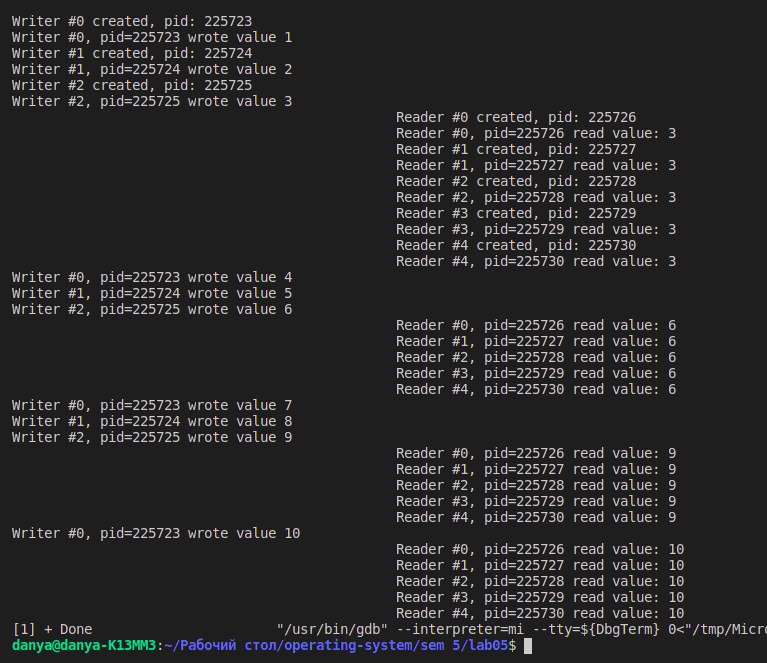
\includegraphics[scale=0.6]{image/task2.jpg}} 
	\caption{Пример работы программы.}
	\label{ris:5}
\end{figure}


\end{document}
